% arara: latexmk: { engine: lualatex, options: [-synctex=1, -aux-directory=./build] }
\documentclass[polish,pretty,bibliography=totocnumbered]{angav}
% [begin] remove when gpoore/minted#467 is fixed
\makeatletter
\let\pdf@mdfivesum\pdf@mdfivesumnative
\makeatother
% [end] remove when gpoore/minted#467 is fixed

\title{Lean \& ITP}
\author{Michał Dobranowski}
\date{\today}

\setmonofont{JetBrainsMono}[Scale=0.85,Contextuals=AlternateOff]  % disable ligatures

\usepackage{ebproof}
\usepackage{stmaryrd} % for \llbracket and \rrbracket
\newcommand{\toto}{\twoheadrightarrow}
\newcommand{\FV}{\opname{FV}}
\newcommand{\Lean}[1]{\mintinline[fontsize=\normalsize]{lean4}{#1}}
\newcommand{\centerLean}[2][]{\begin{center}\Lean{#2}#1\end{center}}

\begin{document}
\maketitle
\tableofcontents
\newpage

\section{Wstęp teoretyczny}

Aby zrozumieć, dlaczego systemowi wspomagającego dowodzenie (ang. \textit{proof assistant}) możemy ufać bardziej niż tuszowi na papierze, należy zrozumieć narzędzia oferowane przez logikę, rachunek lambda oraz teorię typów, na których zbudowany jest każdy znany autorowi tego typu system.
Chociaż ten kurs nigdy nie miał być teoretyczny, zdaniem autora formalizmy dotyczące (typowanego) rachunku lambda są niezwykle ciekawe, więc w odpowiednich miejscach Czytelnik jest zachęcany do pogłębienia wiedzy, w tym też przeprowadzenia lub przeczytania dowodów przytaczanych twierdzeń.

\subsection{Logika intuicjonistyczna}

Typowym przykładem ilustrującym różnicę między logiką klasyczną a intuicjonistyczną (konstruktywną) jest twierdzenie:
\begin{displayquote}
    Istnieją takie liczby niewymierne $a$ i $b$, że $a^b$ jest liczbą wymierną.
\end{displayquote}
oraz jego dowód:
\begin{displayquote}
    Jeśli $\sqrt{2}^{\sqrt{2}} \in \QQ$, to $a = b = \sqrt{2}$, w przeciwnym razie niech $a = \sqrt{2}^{\sqrt{2}}$ oraz $b = \sqrt{2}$, wtedy $a^b = 2 \in \QQ$.
\end{displayquote}
Dowód ten jest oczywiście słuszny na gruncie logiki klasycznej, ale nie jest konstruktywny, ponieważ dalej nie znamy odpowiednich liczb $a$ i $b$. W logice konstruktywnej zdanie jest prawdziwe, jeśli można podać jego \vocab{konstrukcję} (tzn. intuicyjny dowód), zgodnie z interpretacją Brouwera-Heytinga-Kolmogorowa:
\begin{itemize}[noitemsep]
    \item konstrukcja dla $A \land B$ to konstrukcja dla $A$ oraz konstrukcja dla $B$,
    \item konstrukcja dla $A \lor B$ to konstrukcja dla $A$ lub konstrukcja dla $B$ wraz z zaznaczeniem, która z nich to jest,
    \item konstrukcja dla $A \to B$ to przekształcenie każdej konstrukcji dla $A$ w konstrukcję dla $B$,
    \item nie istnieje konstrukcja dla fałszu.
\end{itemize}

Formalnie, logika intuicjonistyczna to pewien system logiczny. Nie różni się od logiki klasycznej składnią, ale regułami wnioskowania.
Fałsz oznaczamy przez $\bot$, a \vocab{osąd} zapisany w postaci $\Gamma \vdash A$ oznacza, że formuła $A$ wynika ze zbioru formuł (założeń) $\Gamma$.
Zamiast $\Gamma \cup \{B\}$ będziemy często pisać $\Gamma, B$.

\begin{figure}[H]
    \[
    \begin{prooftree}
        \infer0[(Ax)]{\Gamma,A\vdash A}
    \end{prooftree}
    \qquad
    \begin{prooftree}
        \hypo{\Gamma\vdash \bot}
        \infer1[($\bot\!$ E)]{\Gamma\vdash A}
    \end{prooftree}
    \]

    \[
    \begin{prooftree}
        \hypo{\Gamma\vdash A}
        \hypo{\Gamma\vdash B}
        \infer2[($\land\!$ I)]{\Gamma\vdash A \land B}
    \end{prooftree}
    \qquad
    \begin{prooftree}
        \hypo{\Gamma\vdash A \land B}
        \infer1[($\land\!$ E1)]{\Gamma\vdash A}
    \end{prooftree}
    \qquad
    \begin{prooftree}
        \hypo{\Gamma\vdash A \land B}
        \infer1[($\land\!$ E2)]{\Gamma\vdash B}
    \end{prooftree}
    \]

    \[
    \begin{prooftree}
        \hypo{\Gamma\vdash A}
        \infer1[($\lor\!$ I1)]{\Gamma\vdash A \lor B}
    \end{prooftree}
    \qquad
    \begin{prooftree}
        \hypo{\Gamma\vdash A}
        \infer1[($\lor\!$ I2)]{\Gamma\vdash B \lor A}
    \end{prooftree}
    \qquad
    \begin{prooftree}
        \hypo{\Gamma\vdash A \lor B}
        \hypo{\Gamma,A\vdash C}
        \hypo{\Gamma,B\vdash C}
        \infer3[($\lor\!$ E)]{\Gamma\vdash C}
    \end{prooftree}
    \]

    \[
    \begin{prooftree}
        \hypo{\Gamma,A\vdash B}
        \infer1[($\to\!$ I)]{\Gamma\vdash A \to B}
    \end{prooftree}
    \qquad
    \begin{prooftree}
        \hypo{\Gamma\vdash A \to B}
        \hypo{\Gamma\vdash A}
        \infer2[($\to\!$ E)]{\Gamma\vdash B}
    \end{prooftree}
    \]
    \caption{Reguły wnioskowania w intuicjonistycznym rachunku zdań (IRZ).}
\end{figure}

Oprócz tego, definiujemy negację jako $\neg A \coloneqq A \to \bot$. Dzięki tej definicji oraz regule ($\to\!$~E) możemy wywieść
\[
\begin{prooftree}
    \hypo{\Gamma\vdash A}
    \hypo{\Gamma\vdash \neg A}
    \infer2[($\neg\!$ E)]{\Gamma\vdash \bot}
\end{prooftree}
\]
Oznaczamy również prawdę przez $\top \coloneqq \neg\bot = \bot \to \bot$.

\begin{example}
    Pokaż, że w IRZ zachodzi \vocab{słabe prawo podwójnej negacji}, czyli $A \to \neg\neg A$.
\end{example}
\begin{solution}
    Z definicji negacji mamy $\neg\neg A = (A \to \bot) \to \bot$, więc musimy pokazać $A \to ((A\to\bot) \to \bot)$.
    \[
    \begin{prooftree}
        \infer0[(Ax)]{A, A\to\bot \vdash A\to\bot}
        \infer0[(Ax)]{A, A\to\bot \vdash A}
        \infer2[($\to\!$ E)]{A, A\to\bot \vdash \bot}
        \infer1[($\to\!$ I)]{A \vdash (A\to\bot) \to \bot}
        \infer1[($\to\!$ I)]{\vdash A \to ((A\to\bot) \to \bot)}
    \end{prooftree}
    \]
\end{solution}

\begin{example}
    Pokaż, że w IRZ zachodzi \vocab{prawo kontrapozycji}, czyli $(A \to B) \to (\neg B \to \neg A)$.
\end{example}
\begin{solution}
    Z definicji negacji mamy $\neg B = B \to \bot$ oraz $\neg A = A \to \bot$, więc musimy pokazać $(A \to B) \to ((B\to\bot) \to (A\to\bot))$.
    \[
    \resizebox{\hsize}{!}{
    \begin{prooftree}
        \infer0[(Ax)]{A\to B, B \to \bot, A \vdash B \to \bot}
        \infer0[(Ax)]{A\to B, B \to \bot, A \vdash A \to B}
        \infer0[(Ax)]{A\to B, B \to \bot, A \vdash A}
        \infer2[($\to\!$ E)]{A \to B, B \to \bot, A \vdash B}
        \infer2[($\to\!$ E)]{A \to B, B \to \bot, A \vdash \bot}
        \infer1[($\to\!$ I)]{A \to B, B \to \bot \vdash A\to\bot}
        \infer1[($\to\!$ I)]{A \to B \vdash (B \to \bot) \to (A \to \bot)}
        \infer1[($\to\!$ I)]{\vdash (A \to B) \to ((B \to \bot) \to (A \to \bot))}
    \end{prooftree}
    }
    \]
\end{solution}

\subsubsection{Związek z logiką klasyczną}

Dokładając do reguł wnioskowania IRZ \vocab{silne prawo podwójnej negacji} ($\neg\neg A \to A$) lub \vocab{prawo wyłączonego środka} ($A \lor \neg A$),  otrzymujemy logikę klasyczną.
W przypadku prawa podwójnej negacji jest to oczywiste. W przypadku prawa wyłączonego środka (EM) można to pokazać następująco:
\[
\resizebox{\hsize}{!}{
\begin{prooftree}
    \infer0[(\textcolor{AccColor1}{EM})]{(A \to \bot) \to \bot \vdash A \lor (A \to \bot)}
    \infer0[(Ax)]{(A \to \bot) \to \bot, A \vdash A}
    \infer0[(Ax)]{\Gamma \vdash (A \to \bot) \to \bot}
    \infer0[(Ax)]{\Gamma \vdash A \to \bot}
    \infer2[($\to\!$ E)]{\Gamma \vdash \bot}
    \infer1[($\bot\!$ E)]{\Gamma \vdash A}
    \infer3[($\lor\!$ E)]{(A \to \bot) \to \bot \vdash A}
    \infer1[($\to\!$ I)]{\vdash (A \to \bot) \to \bot \to A}
\end{prooftree}
}
\]
gdzie $\Gamma = \{(A \to \bot) \to \bot, A \to \bot\}$.

\begin{problem}
    Pokazać, że prawo wyłączonego środka nie jest dowodliwe w IRZ.
\end{problem}

\begin{remark*}[ciekawostka]
    Istnieją tautologie KRZ, które nie są dowodliwe w IRZ, ale po dodaniu do IRZ jako aksjomaty nie prowadzą do logiki klasycznej, tworząc logiki \enquote{pomiędzy} intuicjonistyczną i klasyczną. Przykłady:
    \begin{itemize}
        \item IRZ + $(\neg A \lor \neg\neg A)$\footnote{słabe prawo wyłączonego środka} --- logika Jankova (de Morgana), w której zachodzą wszystkie cztery prawa de Morgana,
        \item IRZ + $((A \to B) \lor (B \to A))$ --- logika Gödla-Dummeta, w której wartościowania formuł można interpretować jako liczby z przedziału $[0,1]$.
    \end{itemize}
\end{remark*}

Skoro zbiór reguł wnioskowania IRZ jest podzbiorem zbioru reguł wnioskowania KRZ, to każda formuła dowodliwa IRZ jest również dowodliwa w KRZ.

\subsubsection{Semantyka}

Trochę zaniedbując formalizmy, skupimy się przez chwilę na wartościowaniach formuł logicznych.
Możemy określić \vocab{semantykę} dla logiki klasycznej, przypisując formułom prawdziwym wartość $1$, a formułom fałszywym wartość $0$ (definiując przy okazji funkcje $\land, \lor, \to$).
Dla logiki intuicjonistycznej jest to trudniejsze, ale i ciekawsze. Pokażemy dwa z (nieskończenie) wielu możliwych sposobów.
Oba z nich są \vocab{algebrami Heytinga}, których nie będziemy tutaj definiować.
Warto jednak wiedzieć, że formuła logiczna jest tautologią IRZ wtedy i tylko wtedy, gdy jest prawdziwa w każdej algebrze Heytinga.

\paragraph{Semantyka topologiczna}
Możemy zdefiniować semantykę za pomocą topologii na $\RR$:
\begin{align*}
    \llbracket \bot \rrbracket &= \emptyset, \\
    \llbracket \top \rrbracket &= \RR, \\
    \llbracket A \land B \rrbracket &= \llbracket A \rrbracket \cap \llbracket B \rrbracket, \\
    \llbracket A \lor B \rrbracket &= \llbracket A \rrbracket \cup \llbracket B \rrbracket, \\
    \llbracket A \to B \rrbracket &= \opname{int}\left(\llbracket A \rrbracket^\complement \cup \llbracket B \rrbracket\right), \\
    \llbracket A \rrbracket &= \text{dowolny otwarty podzbiór $\RR$.}
\end{align*}
Wtedy
\[ \llbracket \neg A \rrbracket = \llbracket A \to \bot \rrbracket = \opname{int}\left(\llbracket A \rrbracket^\complement \cup \emptyset\right) = \opname{int}\left(\llbracket A \rrbracket^\complement\right) \]

Można przy pomocy takiej semantyki pokazać, że prawo wyłączonego środka nie jest dowodliwe w IRZ. Pod $\llbracket A \rrbracket$ możemy podstawić np. zbiór $(0, \infty)$, wtedy
\[ \llbracket A \lor \neg A \rrbracket = \llbracket A \rrbracket \cup \llbracket \neg A \rrbracket = \llbracket A \rrbracket \cup \opname{int}\left(\llbracket A \rrbracket^\complement\right) = (0, \infty) \cup (-\infty, 0) \neq \RR \]

\paragraph{Semantyka kraty dystrybutywnej}
Krata to zbiór częściowo uporządkowany, w którym istnieją kresy dolne i górne dowolnych par elementów.
Będziemy je przedstawiać za pomocą \vocab{diagramów Hassego}\footnote{Czym dokładnie jest diagram Hassego można dowiedzieć się na \href{https://pl.wikipedia.org/wiki/Diagram_Hassego}{Wikipedii}.}.
Definiujemy działania
\begin{align*}
    a \land b &\coloneqq \inf\{a, b\}, \\
    a \lor b &\coloneqq \sup\{a, b\}.
\end{align*}

Krata dystrybutywna to krata, w której zachodzą prawa rozdzielności:
\begin{align*}
    a \land (b \lor c) &= (a \land b) \lor (a \land c), \\
    a \lor (b \land c) &= (a \lor b) \land (a \lor c).
\end{align*}

Można udowodnić, że każda niepusta i skończona krata jest ograniczona, czyli posiada elementy najmniejszy i największy. Krata, która jest niepusta, skończona i dystrybutywna posłuży nam do zdefiniowania semantyki:
\begin{align*}
    \llbracket \bot \rrbracket &= \text{element najmniejszy}, \\
    \llbracket \top \rrbracket &= \text{element największy}, \\
    \llbracket A \land B \rrbracket &= \llbracket A \rrbracket \land \llbracket B \rrbracket, \\
    \llbracket A \lor B \rrbracket &= \llbracket A \rrbracket \lor \llbracket B \rrbracket, \\
    \llbracket A \to B \rrbracket &= \sup\{c : c \land \llbracket A \rrbracket \leq \llbracket B \rrbracket\}, \\
    \llbracket A \rrbracket &= \text{dowolny element kraty.}
\end{align*}
Wtedy
\[ \llbracket \neg A \rrbracket = \llbracket A \to \bot \rrbracket = \sup\{c : c \land \llbracket A \rrbracket \leq \llbracket \bot \rrbracket\} = \sup\{c : c \land \llbracket A \rrbracket = \llbracket \bot \rrbracket\} \]

Biorąc przykładową kratę
\begin{figure}[H]
    \centering
    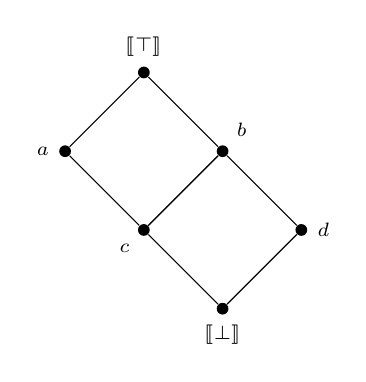
\begin{tikzpicture}[scale=2]
        \tikzset{dot/.style={circle, fill, inner sep=1.5pt}}
        \tikzset{every label/.append style={font=\scriptsize}}

        \node[dot,label=left:$a$]         (B) at (-0.5,0.5) {};
        \node[dot,label=above:$\llbracket \top \rrbracket$] (D) at (0,1) {};
        \node[dot,label=above right:$b$]  (C) at (0.5,0.5) {};
        \node[dot,label=below left:$c$]   (A) at (0,0) {};
        \node[dot,label=right:$d$]        (E) at (1,0) {};
        \node[dot,label=below:$\llbracket \bot \rrbracket$] (F) at (0.5,-0.5) {};

        \draw (B) -- (D) -- (C) -- (A) -- (B);
        \draw (A) -- (C) -- (E) -- (F) -- (A);
    \end{tikzpicture}
\end{figure}
możemy udowodnić, że prawo wyłączonego środka nie jest dowodliwe w IRZ. Jeśli weźmiemy $\llbracket A \rrbracket = c$, to $\llbracket \neg A \rrbracket = d$, więc $\llbracket A \lor \neg A \rrbracket = c \lor d = b \neq \llbracket \top \rrbracket$.

\begin{problem}
    Pokazać, że silne prawo podwójnej negacji nie jest dowodliwe w IRZ na podstawie dwóch powyższych semantyk.
\end{problem}

\begin{problem}
    Stwierdzić, które z czterech praw de Morgana są dowodliwe w IRZ.
\end{problem}

\subsection{Rachunek lambda}

Rachunek lambda to język złożony z termów, z których każdy to:
\begin{itemize}
    \item zmienna (zazwyczaj oznaczana małą literą, np. $x$),
    \item $\lambda$-abstrakcja postaci $\lambda x\ldotp M$, gdzie $x$ jest zmienną, a $M$ jest termem,
    \item aplikacja postaci $MN$, gdzie $M$ i $N$ są termami.
\end{itemize}

Formalnie termy można więc zdefiniować następująco:
\[ M \Coloneqq x \mid (\lambda x\ldotp M) \mid (MM), \]
gdzie $x$ reprezentuje dowolną zmienną.

Aby uprościć zapis, będziemy pisać $MNP$ zamiast $(MN)P$ -- to znaczy stwierdzamy, że aplikacja jest łączna lewostronnie. Ponadto, wiele $\lambda$-abstrakcji zapisujemy jako $\lambda x_1 \ldots x_n\ldotp M$, co jest równoważne termowi $\lambda x_1\ldotp (\lambda x_2\ldotp (\ldots (\lambda x_n\ldotp M) \ldots))$. Kropka w tym zapisie jest bardzo istotna, np.
\begin{align*}
    \lambda xyz\ldotp M &= \lambda x\ldotp (\lambda y\ldotp (\lambda z\ldotp M)), \\
    \lambda xy\ldotp z M &= \lambda x\ldotp (\lambda y\ldotp (z M)).
\end{align*}

W termie $\lambda x\ldotp M$ zmienna $x$ jest \vocab{zmienną związaną} w $M$.
Zmienne występujące w $M$, które nie są związane przez żadną $\lambda$-abstrakcję, nazywamy \vocab{zmiennymi wolnymi}.
Na przykład w termie $\lambda x\ldotp (x y)$ zmienna $x$ jest zmienną związaną, a $y$ jest zmienną wolną.
W termie $xz(\lambda xy\ldotp (xyz))$ zmienna $x$ raz występuje jako zmienna wolna, a raz jako związana. Takich sytuacji będziemy unikać ze względów czysto estetycznych.

Zbiór zmiennych wolnych termu $M$ oznaczamy jako $\FV(M)$.
Term nazywamy \vocab{termem zamkniętym} lub \vocab{kombinatorem}, jeśli $\FV(M) = \emptyset$.

\begin{remark}
    Formalnie definiujemy $\FV(M)$ rekurencyjnie:
    \begin{align*}
        \FV(x) &= \{x\}, \\
        \FV(\lambda x\ldotp M) &= \FV(M) \setminus \{x\}, \\
        \FV(MN) &= \FV(M) \cup FV(N).
    \end{align*}
\end{remark}

\subsubsection{Alfa-konwersja}

\vocab{$\alpha$-konwersja} to przekształcenie termu, które polega na zmianie nazwy zmiennej (unikając kolizji oznaczeń zmiennych). Wprowadzamy relację równoważności $\equiv_\alpha$ w zbiorze termów $\Lambda$ w ten sposób, że dane dwa termy $M$ i $N$ są równoważne, jeśli można otrzymać jeden z drugiego poprzez (wielokrotne) $\alpha$-konwersje. Na przykład:
\[ a (\lambda b\ldotp bc) \equiv_\alpha a (\lambda d\ldotp dc), \]
natomiast
\[ \lambda a\ldotp ab \nequiv_\alpha \lambda b\ldotp bb, \]
ponieważ zamiana zmiennej $a$ na $b$ prowadzi do kolizji oznaczeń zmiennych.

Od tej pory utożsamiamy ze sobą termy różniące się jedynie nazwami zmiennych, czyli jeśli $M \equiv_\alpha N$, to $M$ i $N$ są tym samym termem.

\begin{remark}
    Bardziej formalnie, od tej pory będziemy operować na klasach abstrakcji relacji $\equiv_\alpha$ (elementach zbioru $\Lambda/{\equiv_\alpha}$), podobnie jak przy działaniach modulo operujemy na klasach abstrakcji relacji przystawania modulo $p$ (elementach zbioru $\ZZ/{\equiv_p}$).
\end{remark}

Będziemy stosować dosyć uniwersalny zapis $M[x \coloneqq N]$ na term, który powstał z termu $M$ poprzez zastąpienie wszystkich \emph{wolnych} wystąpień zmiennej $x$ termem $N$.
Zakładamy przy tym, że żadna zmienna wolna w $N$ nie zacznie być związana w $M[x \coloneqq N]$ (ponownie unikamy kolizji oznaczeń).

\subsubsection{Beta-redukcja}

\vocab{$\beta$-redukcja} to taka relacja $\to_\beta$ w zbiorze termów $\Lambda$, że $M \to_\beta N$, gdy \vocab{$\beta$-redeks} postaci $(\lambda x\ldotp P)Q$ w termie $M$ zostaje zastąpiony przez $P[x \coloneqq Q]$ w termie $N$.
Bardziej formalnie, jest to najmniejsza relacja w zbiorze $\Lambda$ spełniająca następujące warunki:
\begin{enumerate}
    \item $(\lambda x\ldotp P)Q \to_\beta P[x \coloneqq Q]$,
    \item jeśli $M \to_\beta M'$, to
    \begin{itemize}[nosep]
        \item $MN \to_\beta M'N$,
        \item $NM \to_\beta NM'$,
        \item $\lambda x\ldotp M \to_\beta \lambda x\ldotp M'$.
    \end{itemize}
\end{enumerate}

Jeśli w termie występuje więcej niż jeden $\beta$-redeks, to $\beta$-redukcja nie jest deterministyczna -- możemy wybrać dowolny z nich i wykonać redukcję.
Przez $\toto_\beta$ oznaczamy domknięcie przechodnio-zwrotne relacji $\to_\beta$ (czyli najmniejsza relacja przechodnia i zwrotna, która zawiera relację $\to_\beta$), a przez $=_\beta$ jej domknięcie równoważnościowe.

\begin{example}
    \label{eq:beta-reduction}
    Pokazane poniżej są różne ścieżki redukcyjne dla podanego termu.
    \tikzset{>={Computer Modern Rightarrow[scale=1.3]}}
    \begin{center}
        \begin{tikzpicture}
            \node (start) at (0, 0) {$\left(\lambda x\ldotp xx\right)\left(\left(\lambda y\ldotp y\right) z\right)$};
            \node (A) at (3, 2) {$\left(\lambda x\ldotp xx\right)z$};
            \node (B) at (2, -2) {$\left(\left(\lambda y\ldotp y\right) z\right)\left(\left(\lambda y\ldotp y\right) z\right)$};
            \node (B2) at (6, -2) {$\left(\left(\lambda y\ldotp y\right) z\right)z$};
            \node (end) at (9, 0) {$zz$};
            \draw[->] (start) to node[above left] {\footnotesize$\beta$} (A);
            \draw[->] (start) to node[below left] {\footnotesize$\beta$} (B);
            \draw[->] (B) to node[below] {\footnotesize$\beta$} (B2);
            \draw[->] (B2) to node[below right] {\footnotesize$\beta$} (end);
            \draw[->] (A) to node[above] {\footnotesize$\beta$} (end);
        \end{tikzpicture}
    \end{center}
\end{example}

\begin{theorem}[Churcha-Rossera]
    Jeśli $M \toto_\beta P$ oraz $M \toto_\beta Q$, to istnieje takie $M'$, że $P \toto_\beta M'$ i $Q \toto_\beta M'$.
\end{theorem}

Jest to jedno z ważniejszych twierdzeń rachunku lambda, mówiące o tym, że relacja $\toto_\beta$ ma \vocab{własność rombu} (ang. \textit{diamond property}), której notabene nie ma relacja $\to_\beta$ (czego dowodzi przykład \ref{eq:beta-reduction}). Jeśli dopełnienie przechodnio-zwrotne relacji ma własność rombu, to mówimy, że relacja ta jest \vocab{konfluentna}. Powyższe twierdzenie mówi więc, że relacja $\to_\beta$ jest konfluentna.

\begin{figure}[H]
    \centering
    \tikzset{>={Computer Modern Rightarrow[scale=1.3]}}
    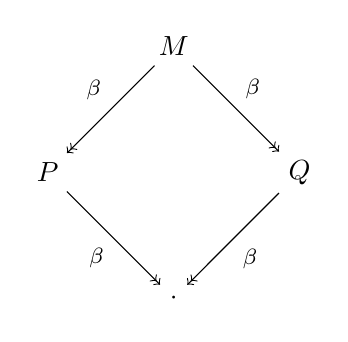
\begin{tikzpicture}[scale=0.8]
        \node (M) at (0, 0) {$M$};
        \node (P) at (-2, -2) {$P$};
        \node (Q) at (2, -2) {$Q$};
        \node (X) at (0, -4) {$\cdot$};
        \draw[->>] (M) to node[above left] {\footnotesize$\beta$} (P);
        \draw[->>] (M) to node[above right] {\footnotesize$\beta$} (Q);
        \draw[->>] (P) to node[below left] {\footnotesize$\beta$} (X);
        \draw[->>] (Q) to node[below right] {\footnotesize$\beta$} (X);
    \end{tikzpicture}
    \caption{Własność rombu relacji $\toto_\beta$.}
    \label{fig:church-rosser}
\end{figure}

Prostym wnioskiem z tego twierdzenia jest fakt, że każdy term ma co najwyżej jedną postać normalną, to znaczy pozbawioną $\beta$-redeksów.
Dlaczego \emph{co najwyżej}, a nie \emph{dokładnie}? Na przykład term
\[ \symbf{\Omega} \coloneqq \left(\lambda x\ldotp xx\right)\left(\lambda x\ldotp xx\right) \]
posiada tylko jeden $\beta$-redeks, a jego redukcja prowadzi do termu $\symbf{\Omega}$ (co Czytelnik raczy sprawdzić), czyli $\symbf{\Omega} \to_\beta \symbf{\Omega}$. Term $\symbf{\Omega}$ nie ma więc postaci normalnej.

\subsubsection{Kombinator punktu stałego}
Kombinator $\symbf{Y} \coloneqq \lambda f\ldotp (\lambda x\ldotp f (xx)) (\lambda x\ldotp f (xx))$ nazywamy \vocab{kombinatorem punktu stałego}. Ma on tę ciekawą własność, że dla każdego termu $F \in \Lambda$, zachodzi
\[ F(\symbf{Y}(F)) =_\beta \symbf{Y}(F), \]
ponieważ
\[ F(\symbf{Y}(F)) \to_\beta F\left((\lambda x\ldotp F (xx)) (\lambda x\ldotp F (xx))\right) \]
oraz
\begin{align*}
    \symbf{Y}(F) &\to_\beta (\lambda x\ldotp F (xx)) (\lambda x\ldotp F (xx)) \\
    &\to_\beta F\left((\lambda x\ldotp F (xx)) (\lambda x\ldotp F (xx))\right).
\end{align*}

\begin{problem}
    Znajdź term $P$ taki, że $Px =_\beta P$.
\end{problem}

\begin{problem}
    Znajdź term $P$ taki, że $Px =_\beta xP$.
\end{problem}

\subsubsection{Eta-redukcja}

\vocab{$\eta$-redukcja} to taka relacja $\to_\eta$ w zbiorze termów $\Lambda$, że $M \to_\eta N$, gdy \vocab{$\eta$-redeks} postaci $\lambda x\ldotp Px$ w termie M zostaje zastąpiony przez $P$ w termie $N$, zakładając $x \notin \FV(P)$.
Bardziej formalnie, jest to najmniejsza relacja w zbiorze $\Lambda$ spełniająca następujące warunki:
\begin{enumerate}
    \item jeśli $x \notin \FV(P)$, to $\lambda x\ldotp Px \to_\eta P$,
    \item jeśli $M \to_\eta M'$, to
    \begin{itemize}[nosep]
        \item $MN \to_\eta M'N$,
        \item $NM \to_\eta NM'$,
        \item $\lambda x\ldotp M \to_\eta \lambda x\ldotp M'$.
    \end{itemize}
\end{enumerate}

Tak jak poprzednio, domknięcie przechodnio-zwrotne relacji $\to_\eta$ oznaczamy przez $\toto_\eta$. Ponadto, sumę relacji $\to_\beta$ i $\to_\eta$ oznaczamy przez $\to_{\beta\eta}$, a jej domknięcie przechodnio-zwrotne przez $\toto_{\beta\eta}$.

\begin{theorem}[Churcha-Rossera dla $\eta$-redukcji i $\beta\eta$-redukcji]
    Relacje $\to_\eta$ oraz $\to_{\beta\eta}$ są konfluentne.
\end{theorem}

\subsubsection{Wyrażalność algorytmów w rachunku lambda}

Liczby naturalne możemy reprezentować w rachunku lambda za pomocą tzw. \vocab{liczebników Churcha}:
\[ \symbf{n} = \lambda fx\ldotp f^n(x), \]
na przykład
\begin{align*}
    \symbf{0} &= \lambda fx\ldotp x, \\
    \symbf{1} &= \lambda fx\ldotp f(x), \\
    \symbf{2} &= \lambda fx\ldotp f(f(x)), \\
    \symbf{3} &= \lambda fx\ldotp f(f(f(x))).
\end{align*}
Wtedy operacja następnika jest reprezentowana przez term
\[ \symbf{succ} = \lambda nfx\ldotp f(nfx), \]
a dodawanie przez term
\[ \symbf{add} = \lambda mnfx\ldotp mf(nfx). \]
Instrukcje warunkowe można zaimplementować za pomocą termów
\[ \symbf{true} = \lambda xy\ldotp x, \]
\[ \symbf{false} = \lambda xy\ldotp y, \]
wtedy instrukcja warunkowa \texttt{if B then M else N} jest reprezentowana przez term
\[ \symbf{if} = \lambda B M N\ldotp B M N. \]
Istotnie,
\begin{align*}
    \symbf{if}\ \symbf{true}\ M\ N &\to_\beta (\lambda xy\ldotp x) M N \to_\beta M, \\
    \symbf{if}\ \symbf{false}\ M\ N &\to_\beta (\lambda xy\ldotp y) M N \to_\beta N.
\end{align*}
Porównanie liczby $n$ do zera można zaimplementować za pomocą termu
\[ \symbf{iszero} = \lambda n\ldotp n (\lambda x\ldotp \symbf{false})\ \symbf{true}. \]

\begin{problem}
    Zdefiniuj w rachunku lambda negację, koniunkcję, alternatywę oraz implikację.
\end{problem}

\begin{problem}
    Zdefiniuj w rachunku lambda funkcje mnożenia oraz potęgowania liczb naturalnych.
\end{problem}

\begin{problem}
    Zdefiniuj w rachunku lambda funkcję poprzednika liczby naturalnej. Poprzednik zera powinien zwracać zero.
\end{problem}

\begin{problem}
    Zdefiniuj w rachunku lambda funkcję obliczającą $n!$.
\end{problem}

\begin{theorem}[Kleene'a]
    Każda funkcja częściowo rekurencyjna jest reprezentowalna w rachunku lambda.
\end{theorem}
Twierdzenie odwrotne również jest prawdziwe. Funkcje częściowo rekurencyjne to dokładnie te funkcje, które są obliczalne przez maszyny Turinga. Z powyższego twierdzenia wynika więc, że rachunek lambda jest modelem obliczalności równoważnym maszynom Turinga.

\subsection{Typowany rachunek lambda}

Do rachunku lambda będziemy chcieli dodać typy w następujący sposob. Każdy term rachunku lambda będzie miał przypisany pewien typ, co będziemy zapisywać jako $M : \tau$, gdzie $M$ jest termem, a $\tau$ jest typem. Niech $\symbb{A}$ będzie zbiorem \vocab{typów atomowych}. Zbiór wszystkich typów $\symbb{T}$ definiujemy rekurencyjnie:
\begin{align*}
    \alpha &\in \symbb{A} \implies \alpha \in \symbb{T}, \\
    \sigma, \tau &\in \symbb{T} \implies (\sigma \to \tau) \in \symbb{T},
\end{align*}
gdzie druga reguła jest \vocab{konstruktorem typów funkcyjnych}. Zakładamy przy tym, że nie istnieją typy $\alpha, \beta, \gamma \in \symbb{A}$ takie, że $\alpha \to \beta = \gamma$. Zamiast pisać $\sigma \to (\tau \to \rho)$, będziemy pisać $\sigma \to \tau \to \rho$ (operator $\to$ jest łączny prawostronnie).

\begin{figure}[H]
    \[
    \begin{prooftree}
        \infer0[(Ax)]{\Gamma,x:A\vdash x:A}
    \end{prooftree}
    \]
    \[
    \begin{prooftree}
        \hypo{\Gamma,x:A\vdash M:B}
        \infer1[($\lambda$ abs)]{\Gamma\vdash \lambda x\ldotp M:(A\to B)}
    \end{prooftree}
    \qquad
    \begin{prooftree}
        \hypo{\Gamma\vdash M:(A \to B)}
        \hypo{\Gamma\vdash N:A}
        \infer2[($\lambda$ app)]{\Gamma\vdash MN:B}
    \end{prooftree}
    \]
    \caption{Reguły przypisania typów.}
\end{figure}

\begin{example}
    Niech $\symbb{A} = \{\alpha\}$. Wtedy term $\symbf{true} = \lambda x\ldotp \lambda y\ldotp x$ ma typ $\alpha \to \alpha \to \alpha$, ponieważ
    \[
    \begin{prooftree}
        \infer0[(Ax)]{x:\alpha,y:\alpha\vdash x:\alpha}
        \infer1[($\lambda$ abs)]{x:\alpha\vdash \lambda y\ldotp x:\alpha \to \alpha}
        \infer1[($\lambda$ abs)]{\vdash \lambda x\ldotp \lambda y\ldotp x:\alpha \to \alpha \to \alpha}
    \end{prooftree}
    \]
    Oznaczając $\alpha \to \alpha \to \alpha$ przez $\symbb{B}$ (typ boolowski), możemy pokazać, że term $\symbf{neg}\ \symbf{true}$ również ma typ $\symbb{B}$.
\end{example}

\subsubsection{Izomorfizm Curry'ego-Howarda}

Pokazany powyżej system typów możemy rozszerzyć o konstruktory typów $\land$ i $\lor$ oraz dodać do $\symbb{A}$ specjalny typ $\bot$, który nie będzie przypisany żadnemu termowi.
Reguły przypisania typów należałoby wtedy rozszerzyć o odpowiednie zasady konstrukcji i destrukcji dla tych nowych typów.

Izomorfizm Curry'ego-Howarda to twierdzenie, które łączy logikę i tak zbudowaną teorię typów.
Mówi ono, że jeśli formułom logicznym przypiszemy odpowiednie typy, a dowodom tych formuł przypiszemy odpowiednie termy, to otrzymamy izomorfizm postaci:
\[ \text{formuła ma dowód} \iff \text{typ ma term}. \]
W ten sposób możemy przepisać formułę logiczną do postaci typu i udowodnić ją, konstruując term tego typu.
W tym właśnie procesie przydaje się oprogramowanie takie jak Lean.

\begin{table}[H]
    \centering
    \begin{tabular}{ll}
        \hline
        logika intuicjonistyczna & typowany rachunek lambda \\
        \hline
        formuła $A$ & typ $A \in \symbb{T}$ \\
        dowód formuły $A$ & term typu $A$ \\
        implikacja & typ funkcyjny ($\to$) \\
        formuła niedowodliwa & typ nieposiadający termu \\
        tautologia & typ kombinatora \\
        \hline
    \end{tabular}
    \caption{Odpowiadające sobie pojęcia w logice i w typowanym rachunku lambda.}
\end{table}

\section{Podstawy dowodzenia w Lean}

Polecam używać VS Code z rozszerzeniem \textbf{Lean 4} lub Neovim z rozszerzeniem \textbf{lean.nvim}.
Aby rozpocząć pracę, należy stworzyć projekt za pomocą
\begin{minted}{bash}
lake new project-name math-lax
\end{minted}
który od razu dodaje Mathlib (de facto bibliotekę standardową, zawierającą wiele twierdzeń z różnych działów matematyki) do wymaganych zależności.

\subsection{Składnia -- bardzo krótki wstęp}

Póki co nie będziemy się zagłębiać w składnię, a jedynie wymienimy kilka podstawowych elementów, które posłużą nam do w miarę swobodnego poruszania się w Leanie (a przynajmniej jego części dotyczącej dowodzenia twierdzeń matematycznych).

\subparagraph{Funkcje i stałe}
Funkcje (oraz stałe, które są funkcjami stałej wartości) definiujemy za pomocą słowa kluczowego \Lean{def}, na przykład:
\begin{minted}{lean4}
def add (a b : Nat) : Nat := a + b
\end{minted}
definiuje funkcję \Lean{add}, która przyjmuje dwie liczby naturalne (typ \Lean{Nat}) i zwraca ich sumę.

\subparagraph{Twierdzenia i przykłady}
Twierdzenia definiujemy za pomocą słowa kluczowego \Lean{theorem} lub \Lean{lemma}, na przykład:
\begin{minted}{lean4}
theorem add_zero (a : Nat) : add a 0 = a := -- dowód
\end{minted}
przy czym używanie \Lean{lemma} wymaga dodania Mathliba (\Lean{import Mathlib.Tactic}).
Jeśli mamy pewne stwierdzenie (z dowodem), którego nie będziemy używać, więc nie potrzebuje nazwy, możemy użyć słowa kluczowego \Lean{example}:
\begin{minted}{lean4}
example (a : Nat) : add 0 a = a := -- dowód
\end{minted}
Samo sformułowanie twierdzeń, lematów i przykładów jest często pewną trudnością. Możemy być więc w sytuacji, gdy chcemy najpierw sformułować tezę, a jej dowód zostawić na później.
W takim przypadku nieodzowne będzie słowo kluczowe \Lean{sorry}, dzięki któremu program się skompiluje (z ostrzeżeniem), mimo braku dowodu.
\begin{minted}{lean4}
theorem pow_comm (a b : Nat) : a ^ b = b ^ a :=
  sorry
\end{minted}
Oczywiście, taka teza może być fałszywa (jak powyżej).

\begin{remark}[Plausible]
    Istnieje paczka Leana o nazwie \textbf{Plausible}, która pomaga w szybkim szukaniu kontrprzykładów do hipotez. Jej działania opiera sie po prostu na losowym próbkowaniu argumentów i sprawdzaniu, czy teza zachodzi. Jeśli nie, to zwraca znaleziony kontrprzykład (przez informację diagnostyczną błędu kompilacji).
    \begin{minted}{lean4}
import Plausible

theorem pow_comm (a b : Nat) : a ^ b = b ^ a := by
  plausible
    \end{minted}
\end{remark}

\subparagraph{Aksjomaty}
Czasami będziemy chcieli wprowadzić pewne aksjomaty, czyli stwierdzenia przyjmowane bez dowodu. W tym celu używamy słowa kluczowego \Lean{axiom}:
\begin{minted}{lean4}
axiom add_comm (a b : Nat) : a + b = b + a
\end{minted}

\subparagraph{Komentarze}
Komentować kod można i należy następująco:
\begin{minted}{lean4}
def foo : Nat := 42 -- to jest komentarz jednowierszowy
/- to jest
komentarz
wielowierszowy -/
\end{minted}

\subparagraph{Sprawdzenie typu}
Sprawdzić typ termu (czyli, przez izomorfizm Curry'ego-Howarda, również wypowiedź twierdzenia), możemy następująco:
\begin{minted}{lean4}
#check Nat -- Nat : Type
#check Nat.add -- Nat.add : Nat → Nat → Nat
#check Nat.add 1 -- Nat.add 1 : Nat → Nat
#check Nat.add 1 2 -- Nat.add 1 2 : Nat
#check Nat.add_comm -- Nat.add_comm (n m : Nat) : n + m = m + n
\end{minted}

\begin{problem}
    \label{prob:type-of-type}
    Skoro \Lean{Nat} jest typu \Lean{Type}, to jaki jest typ \Lean{Type}? Jaki jest typ tego typu?
\end{problem}

\subparagraph{Ewaluacja funkcji}
Czasami, zamiast dowodzić twierdzeń, będziemy chcieli po prostu obliczyć wartość pewnej funkcji. Możemy to zrobić tak:
\begin{minted}{lean4}
#eval Nat.add 2 3 -- 5
\end{minted}

\subparagraph{Operatory potoku i odwróconego potoku}
Jak na porządny język programowania przystało, Lean posiada operatory umożliwiające kontrolę kolejności ewaluacji wyrażeń. Operatory \texttt{<|} i \texttt{|>} zachowują się tak samo jak w F\# czy Elm, sam operator \texttt{|>} znajdziemy również w Elixirze czy OCaml-u.
W Haskellu odpowiadają one odpowiednio operatorom \texttt{\$} i \texttt{\&}. Przykłady użycia:
\begin{minted}{lean4}
#eval Nat.add 1 (Nat.mul 2 3)   -- 7
#eval Nat.add 1 <| Nat.mul 2 3  -- 7
#eval Nat.mul 2 3 |> Nat.add 1  -- 7
\end{minted}

\subsubsection{Tryby dowodzenia}

Dowodząc twierdzenie, lemat, czy przykład, możemy wybrać jeden z dwóch trybów:
\begin{itemize}
    \item \vocab{tryb termowy} (ang. \textit{term mode}), w którym dowód jest pojedynczym (potencjalnie długim) termem,
    \item \vocab{tryb taktyczny} (ang. \textit{tactic mode}), w którym dowód jest ciągiem \vocab{taktyk} modyfikujących stan dowodu.
\end{itemize}
Pierwszy jest zbliżony do rachunku lambda, drugi bardziej przypomina tradycyjne dowodzenie matematyczne. Często proste fakty łatwiej udowodnić w trybie termowym, a bardziej złożone w trybie taktycznym.
Oto przykład dowodu (a właściwie zastosowania twierdzenia) w obu trybach:
\begin{minted}{lean4}
-- term mode (aplikacja 2a i 2b do twierdzenia Nat.add_comm)
example (a b : Nat) : 2 * a + 2 * b = 2 * b + 2 * a := Nat.add_comm (2 * a) (2 * b)
-- tactic mode (po by następuje taktyka rw)
example (a b : Nat) : 2 * a + 2 * b = 2 * b + 2 * a := by rw [Nat.add_comm]
\end{minted}

\subsubsection{Argumenty i ich rodzaje}

Czytelnik już zapewne zdążył zauważyć, że twierdzenia w Leanie zazwyczaj przyjmują argumenty. Na przykład w twierdzeniu \Lean{Nat.add_comm} mamy argumenty \Lean{(n : Nat)} i \Lean{(m : Nat)}, zapisywane jako \Lean{(n m : Nat)}.
Takimi argumentami będą również założenia twierdzenia, na przykład w:
\begin{minted}{lean4}
theorem tw (a : Nat) (b : Nat) (c : Nat) (h₁ : a < b) (h₂ : b < c) : a < c := sorry
\end{minted}
Chcąc użyć takiego twierdzenia, musimy podać wszystkie argumenty, np.
\begin{minted}{lean4}
axiom one_lt_two : 1 < 2
axiom two_lt_three : 2 < 3

#check tw 1 2 3 one_lt_two two_lt_three
\end{minted}

Widać tutaj więc pewną redundancję -- argumenty \Lean{a}, \Lean{b} i \Lean{c} są w pełni określone przez założenia \Lean{h₁} i \Lean{h₂}.
Aby tego uniknąć, Lean pozwala na definiowanie argumentów \textit{implicit}, czyli takich, które mogą być pominięte przy wywoływaniu danej funkcji lub twierdzenia. W tym celu używamy nawiasów klamrowych zamiast okrągłych:
\begin{minted}{lean4}
theorem tw {a : Nat} {b : Nat} {c : Nat} (h₁ : a < b) (h₂ : b < c) : a < c := sorry
\end{minted}
Teraz możemy użyć tego twierdzenia jako
\begin{minted}{lean4}
#check tw one_lt_two two_lt_three
\end{minted}

Oprócz argumentów \textit{explicit} i \textit{implicit}, Lean pozwala na definiowanie argumentów \textit{instance implicit} oraz \textit{strict implicit}, oznaczanych odpowiednio przez $[\ldots]$ oraz $⦃\ldots⦄$. Zajmiemy się nimi później.

\subsubsection{Typy Sort, Type i Prop}

W ramach problemu \ref{prob:type-of-type} Czytelnik miał okazję zastanowić się nad typami \Lean{Type}, \Lean{Type 1}, \Lean{Type 2} itd.
Są one częścią nieskończonej hierarchii typów \Lean{Sort u}, gdzie \Lean{u} jest zmienną uniwersalną oznaczającą poziom uniwersum.
Typ \Lean{Sort u} jest więc typu \Lean{Sort (u + 1)}.
\Lean{Type u} jest synonimem dla \Lean{Sort (u + 1)}, a \Lean{Prop} jest synonimem dla \Lean{Sort 0}.

Skąd takie przesunięcie? Typy typu \Lean{Type u} (a więc sorty poziomu co najmniej 1) \enquote{trzymają} pewne obiekty matematyczne, np. term (liczba) $1$ jest \enquote{trzymana} przez typ \Lean{Nat : Type 0}.
Typy typu \Lean{Prop} (czyli sorty poziomu 0) nie \enquote{trzymają} nic. Tego typu będą więc twierdzenia, od których nie wymagamy (albo nawet nie chcemy), żeby trzymały swój dowód (\textit{proof irrelevance}).

\subsection{Rachunek zdań i pierwsze taktyki}

Od tego miejsca będziemy stosować logikę klasyczną. Jak Lean radzi sobie z rozbieżnościami między logiką intuicjonistyczną a klasyczną? Definiuje aksjomat wyboru:
\centerLean[,]{axiom Classical.choice {α : Sort u} : Nonempty α → α}
z którego następnie, dzięki twierdzeniu Diaconescu, wyprowadza prawo wyłączonego środka \Lean{Classical.em} oraz wiele innych praw logiki klasycznej, jak chociażby silne prawo podwójnego przeczenia \Lean{Classical.not_not}. Niżej omawiane taktyki Leana korzystają z tych aksjomatów, gdy jest to konieczne.

\subparagraph{Taktyki \texttt{intro}, \texttt{exact} i \texttt{apply}}
Jeśli cel dowodzenia znajduje się wśród założeń, to wystarczy go wskazać za pomocą taktyki \Lean{exact}. Jeśli cel jest w postaci \Lean{P → Q}, to możemy użyć taktyki \Lean{intro}, aby wprowadzić do dowodu założenie \Lean{P} i zmienić cel na \Lean{Q}.
\begin{minted}{lean4}
example {P : Prop} (h : P) : P := by
  exact h

example {P : Prop} : P → P := by
  intro h
  exact h
\end{minted}

Jeśli celem jest \Lean{Q}, a mamy wśród założeń \Lean{P → Q}, to możemy użyć taktyki \Lean{apply}, aby zmienić cel na \Lean{P}. Możemy stosować również aplikację znaną z typowanego rachunku lambda.
\begin{minted}{lean4}
example {P Q : Prop} (h₁ : P → Q) (h₂ : P) : Q := by
  apply h₁
  exact h₂

example {P Q : Prop} (h₁ : P → Q) (h₂ : P) : Q := by
  exact h₁ h₂
\end{minted}

\subparagraph{Koniunkcja}
W Lean istnieje struktura \Lean{And}, której jedynym konstrukturem jest
\centerLean[.]{And.intro {a b : Prop} (left : a) (right : b) : a ∧ b}
Jako że \Lean{And.intro} ma typ \Lean{a → b → a ∧ b}, to świetnie nadaje się do użycia z \Lean{apply}, które wprowadzi dwa cele (do rozwiązania jeden po drugim).

Jeśli chcemy w ten sposób użyć konstruktora dowolnej struktury, to możemy użyć taktyki \Lean{constructor}.

\begin{minted}{lean4}
example {P Q : Prop} (hp : P) (hq : Q) : P ∧ Q := by
  apply And.intro
  · exact hp
  · exact hq

example {P Q : Prop} (hp : P) (hq : Q) : P ∧ Q := by
  constructor
  · exact hp
  · exact hq

example {P Q : Prop} (h : P ∧ Q) : P := by
  exact h.left
\end{minted}


\subparagraph{Równoważność}
Struktura \Lean{Iff}, która reprezentuje równoważność logiczną, ma konstruktor
\centerLean[,]{Iff.intro {a b : Prop} (mp : a → b) (mpr : b → a) : a ↔ b}
gdzie pierwszy argument to \textit{modus ponens} ($a \implies b$), a drugi to \textit{modus ponens reversed} ($b \implies a$). Sposób użycia jest analogiczny jak w przypadku koniunkcji. Na przykład
\begin{minted}{lean4}
example {P Q : Prop} (h : P ↔ Q) : Q → P := by
  exact h.mpr
\end{minted}

\subparagraph{Alternatywa}
Istnieje również struktura \Lean{Or}, której konstruktorami są
\centerLean{inl {a b : Prop} (h : a) : a ∨ b}
oraz
\centerLean[.]{inr {a b : Prop} (h : b) : a ∨ b}
Aby ich użyć, skorzystamy z taktyki \Lean{cases} lub \Lean{rcases} (które rekurencyjnie wywołuje \Lean{cases} zgodnie z podanym wzorem).
\begin{minted}{lean4}
example {P Q R : Prop} (hpq : P ∨ Q) (hpr : P → R) (hqr : Q → R) : R := by
  cases hpq with
  | inl hp =>
    apply hpr
    exact hp
  | inr hq =>
    apply hqr
    apply hq

example {P Q R : Prop} (hpq : P ∨ Q) (hpr : P → R) (hqr : Q → R) : R := by
  rcases hpq with hp | hq
  · apply hpr
    exact hp
  · apply hqr
    apply hq
\end{minted}

Taktyka \Lean{rcases} może się przydać również przy koniunkcjach i bardziej złożonych zdaniach, na przykład:
\begin{minted}{lean4}
example {P Q R S : Prop} (h : S ∧ R ∧ P ∨ S ∧ (Q ∧ R)) : R := by
  rcases h with ⟨_, hr, _⟩ | ⟨_, ⟨_, hr⟩⟩
  · exact hr
  · exact hr
\end{minted}

Jeśli alternatywa jest naszym celem, a nie założeniem, to przydatne będą taktyki \Lean{left} i \Lean{right}.

\begin{minted}{lean4}
example {P Q : Prop} (h : P) : P ∨ Q := by
  left
  exact h
\end{minted}

\begin{remark}
    Bardziej dokładnie, taktyka \Lean{constructor} używa pierwszego pasującego konstruktora struktury, a taktyki \Lean{left} i \Lean{right} używają odpowiednio pierwszego i drugiego konstruktora struktury, która ma dokładnie dwa konstruktory. Nie są one przypisane do struktur \Lean{And} i \Lean{Or}. W szczególności, zamiast \Lean{left} zawsze można używać \Lean{constructor}, ale sensowność takiego działania pozostawiamy do oceny Czytelnikowi.
\end{remark}

\subparagraph{Negacja}
Podobnie jak w IRZ, \Lean{¬P} definiujemy jako \Lean{P → False}, gdzie \Lean{False} jest typem bez termów (i bez konstruktora). Bardzo łatwo jest więc dowieść, że $\neg (P \land \neg P)$.
\begin{minted}{lean4}
example (P : Prop) : ¬(P ∧ ¬P) := by
  intro h
  exact h.right h.left
\end{minted}

Z fałszu możemy oczywiście dowieść wszystko. W Leanie \textit{ex falso quodlibet} jest realizowane przez \Lean{False.elim} lub \Lean{absurd}.
\begin{minted}{lean4}
example {P Q : Prop} (h : P) (nh : ¬P) : Q := by
  exact False.elim (nh h)
\end{minted}

\begin{minted}{lean4}
example {P Q : Prop} (h : P) (nh : ¬P) : Q := by
  exact absurd h nh
\end{minted}


\subparagraph{Taktyki \texttt{assumption}, \texttt{contradiction}, \texttt{trivial} oraz operator \texttt{<;>}}
Poniższy przykład (reguła \textit{modus tollendo ponens}) Czytelnik powinien już być w stanie zrozumieć. Pokażemy, jak udowodnić go trochę prościej.
\begin{minted}{lean4}
example {P Q : Prop} (h : P ∨ Q) (not_p : ¬P) : Q := by
  rcases h with hp | hq
  · exact False.elim (not_p hp)
  · exact hq
\end{minted}

Zamiast \Lean{exact hq} możemy użyć taktyki \Lean{assumption}, która sprawdza, czy cel jest wśród założeń (nie musimy go wskazywać). Zamiast \Lean{False.elim} możemy użyć taktyki \Lean{contradiction}, która sprawdza, czy wśród założeń znajdują się dwa trywialne sprzeczne stwierdzenia.
\begin{minted}{lean4}
example {P Q : Prop} (h : P ∨ Q) (not_p : ¬P) : Q := by
  rcases h with hp | hq
  · contradiction
  · assumption
\end{minted}

Jeśli nie używamy wprowadzonych założeń (w przykładzie \Lean{hp} i \Lean{hq}), to nie musimy ich nazywać -- dalej będą one dostępne dla taktyk \Lean{assumption} i \Lean{contradiction}.
\begin{minted}{lean4}
example {P Q : Prop} (h : P ∨ Q) (not_p : ¬P) : Q := by
  cases h
  · contradiction
  · assumption
\end{minted}

Istnieje również taktyka \Lean{trivial}, która próbuje rozwiązać cel używając kilku prostych taktyk, jak \Lean{assumption}, \Lean{contradiction} czy \Lean{rfl} (użyteczna przy równościach).
\begin{minted}{lean4}
example {P Q : Prop} (h : P ∨ Q) (not_p : ¬P) : Q := by
  cases h
  · trivial
  · trivial
\end{minted}

Jeśli chcemy użyć tej samej taktyki dla różnych przypadków, to możemy użyć \Lean{<;>} w następujący sposób:
\begin{minted}{lean4}
example {P Q : Prop} (h : P ∨ Q) (not_p : ¬P) : Q := by
  cases h <;> trivial
\end{minted}

\begin{problem}
    Zrobić pierwszy zestaw zadań:
    \inputminted{lean4}{problemsets/problemset01.lean}
\end{problem}

\subsection{Przekształcenia algebraiczne i równości}

Jeśli nasz cel jest trywialną równością, możemy użyć taktyki \Lean{rfl} (od ang. \textit{reflexivity}).
\begin{minted}{lean4}
example (a : Nat) : a = a := by
  rfl

example : 1 + 1 = 2 := by
  rfl
\end{minted}

Jeśli nasz cel nie jest równością, ale wymaga jedynie \emph{obliczenia}, a nie dowodu (jak w drugim przykładzie powyżej), wystarczy użyć taktyki \Lean{decide}.
\begin{minted}{lean4}
example : 2 * 3 + 1 ≥ 4 := by
  decide
\end{minted}

Często jednak będziemy chcieli użyć jakiejś równości do zmiany fragmentu bardziej skomplikowanej formuły. W tym celu możemy użyć taktyki \Lean{rewrite}, lub \Lean{rw}, która działa jak \Lean{rewrite}, ale próbuje użyć jeszcze \Lean{rfl}.
\begin{minted}{lean4}
example (h : a = b) : a^3 + 1 = b^3 + 1 := by
  rewrite [h]
  rfl

example (h : a = b) : a^3 + 1 = b^3 + 1 := by
  rw [h]
\end{minted}
Domyślnie te taktyki przepisują lewą stronę równości na prawą. Aby przepisać w drugą stronę, należy użyć \Lean{←} przed nazwą równości.
\begin{minted}{lean4}
example {a b c : Nat} (h₁ : 2 * b = a) (h₂ : b = 2 * c) : a = 4 * c := by
  rewrite [←h₁]
  rewrite [h₂]
  rewrite [←Nat.mul_assoc]
  rfl

example {a b c : Nat} (h₁ : 2 * b = a) (h₂ : b = 2 * c) : a = 4 * c := by
  rw [←h₁, h₂, ←Nat.mul_assoc]
\end{minted}
Jeśli chcemy przepisać nie część celu, a któregoś z założeń, wystarczy go wskazać za pomocą \Lean{at}. Możemy też przepisywać kilka formuł naraz, oddzielając je spacjami, gdzie cel oznaczamy przez \Lean{⊢}.
\begin{minted}{lean4}
example {a b c : Nat} (h₁ : 2 * b = a) (h₂ : b = 2 * c) : a = 4 * c := by
  rw [h₂, ←Nat.mul_assoc] at h₁
  rw [h₁]

example {a b : Nat} (h_eq : a = b + 1) (h : a + b = 4) : 2 * a = 5 := by
  rw [h_eq] at h ⊢
  rw [Nat.two_mul]
  rw [←Nat.add_assoc (b + 1) b 1]
  rw [h]
\end{minted}

Bardzo często będziemy chcieli udowodnić najpierw jakiś cel pośredni, żeby następnie wykorzystać go do udowodnienia głównego celu. W takiej sytuacji nie trzeba definiować nowego lematu, a wystarczy użyć taktyki \Lean{have}.
\begin{minted}{lean4}
example {a : Nat} : a * 2 + 1 = 2 * a + 1 := by
  -- h₁, h₂, h₃ to identyczne założenia
  have h₁ : a * 2 = 2 * a := by rw [Nat.mul_comm]
  have h₂ : a * 2 = 2 * a := Nat.mul_comm a 2
  have h₃ := Nat.mul_comm a 2
  apply Nat.add_left_inj.mpr
  assumption

\end{minted}
Takie założenie działa jak każde inne twierdzenie, możemy je więc udowodnić w trybie termowym lub taktycznym.
Jeśli udowadniamy je w trybie termowym, to oczywiście nie musimy nawet formułować jego pełnej treści.
Możemy po \Lean{have} nie dać żadnej nazwy, wtedy Lean automatycznie nazwie to założenie \Lean{this}.

\subsection{Rachunek kwantyfikatorów}

\subparagraph{Kwantyfikator uniwersalny}
Z kwantyfikatora $\forall$ korzystaliśmy już wielokrotnie, chociaż niebezpośrednio. Na przykład twierdzenie $\forall x \in \mathbb{N} (x + 0 = x)$ zapisywaliśmy jako
\begin{minted}{lean4}
theorem add_zero (x : Nat) : x + 0 = x := sorry
\end{minted}
Możemy je również zapisać i udowodnić jako
\begin{minted}{lean4}
theorem add_zero' : ∀ x : Nat, x + 0 = x := by
  intro x
  exact add_zero x
\end{minted}
korzystając z poznanej już taktyki \Lean{intro}. Przeciwieństwem \Lean{intro} w tym kontekście jest taktyka \Lean{revert}, która przenosi podaną zmienną z założeń do kwantyfikatora $\forall$ w celu.

\subparagraph{Kwantyfikator egzystencjalny}
Formuły z kwantyfikatorem $\exists$ najlepiej dowodzić za pomocą dostępnej w \Lean{Mathlib.Tactic.Use} taktyki \Lean{use}.
\begin{minted}{lean4}
example : ∃ n : Nat, n > 1000 := by
  use 1001
  decide
\end{minted}

\begin{problem}
    Dowiedzieć się, jak działa kwantyfikator $\exists!$ w Leanie (zdefiniowany w pliku \Lean{Mathlib.Logic.ExistsUnique}).
\end{problem}

\begin{problem}
    Zrobić drugi zestaw zadań:
    \inputminted{lean4}{problemsets/problemset02.lean}
\end{problem}

\subsection{Taktyki automatyzujące dowodzenie}

Lean posiada wiele taktyk automatyzujących dowodzenie, z których najważniejsze omówimy w tej sekcji.

Udowodnijmy, że dla każdych $a, b \in \NN$ zachodzi $(a + b)^2 = a^2 + 2ab + b^2$.

\begin{minted}{lean4}
example {a b : Nat} : (a + b)^2 = a^2 + 2 * a * b + b^2 := by
  rw [Nat.pow_two]
  rw [Nat.mul_add]
  rw [Nat.add_mul]
  rw [Nat.add_mul]
  rw [←Nat.pow_two]
  rw [←Nat.pow_two]
  rw [←Nat.add_assoc]
  rw [Nat.mul_comm]
  rw [Nat.add_assoc (a^2)]
  rw [←Nat.two_mul]
  rw [Nat.mul_assoc]
\end{minted}

Aby udowadniać podobne tożsamości w pierścieniach przemiennych oraz półpierścieniach przemiennych (na przykład w $\NN$), możemy użyć taktyki \Lean{ring}.
\begin{minted}{lean4}
import Mathlib.Tactic.Ring

example {a b : Nat} : (a + b)^2 = a^2 + 2 * a * b + b^2 := by
  ring
\end{minted}

Jeśli nie chcemy od razu udowadniać równości, a jedynie uprościć cel (np. nierówność), zamiast \Lean{ring} możemy użyć taktyki \Lean{ring_nf} (od ang. \textit{normal form}).

\subsection{Typy zależne, klasy typów, instancje}

\subsection{Indukcja matematyczna}

\todo[inline]{zrobić}

\begin{thebibliography}{9}
    \bibitem{Barendregt2013} H. Barendregt, W. Dekkers, R. Statman, Lambda Calculus with Types, \textit{Perspectives in Logic}, Cambridge University Press, 2013.
    \bibitem{CsirmazGyenis} L. Csirmaz, Z. Gyenis, Mathematical Logic: Exercises and Solutions, \textit{Problem Books in Mathematics}, Springer, 2022.
    \bibitem{SorensenUrzyczyn} M. H. Sørensen, P. Urzyczyn, Lectures on the Curry-Howard Isomorphism, \textit{Studies in Logic and the Foundations of Mathematics}, vol. 149, Elsevier, 2006.
\end{thebibliography}

\end{document}
